\documentclass[conference]{IEEEtran}
\IEEEoverridecommandlockouts

\usepackage{amsmath,amssymb}
\usepackage{graphicx}
\usepackage{booktabs}
\usepackage{xcolor}
\usepackage[hidelinks]{hyperref}
\usepackage{url}

% Every result below comes from generated/macros.tex and generated/tab_*.tex (see make_tables.py).
% Generated by paper/make_tables.py from results_real; do not edit.
\newcommand{\Model}{gpt-4.1-mini}
\newcommand{\Nseeds}{10}
\newcommand{\Npairs}{40}
\newcommand{\BadRate}{0.5}
\newcommand{\GainRule}{0.4}
\newcommand{\IneffRule}{98}
\newcommand{\AccRule}{28}
\newcommand{\TokensRule}{0}
\newcommand{\FalseAlarmRule}{10}
\newcommand{\InvalidRule}{0}
\newcommand{\ExplRule}{2.23}
\newcommand{\StepsRule}{0.0}
\newcommand{\HarmCatchRule}{0}
\newcommand{\HarmNRule}{8}
\newcommand{\AccScnBreakdownsRule}{0}
\newcommand{\GainScnBreakdownsRule}{0.2}
\newcommand{\AccScnBufferRule}{10}
\newcommand{\GainScnBufferRule}{0.6}
\newcommand{\AccScnHealthyRule}{90}
\newcommand{\GainScnHealthyRule}{0.0}
\newcommand{\AccScnMixedRule}{0}
\newcommand{\GainScnMixedRule}{0.5}
\newcommand{\AccScnSlowRule}{100}
\newcommand{\GainScnSlowRule}{0.1}
\newcommand{\GainToc}{13.5}
\newcommand{\IneffToc}{0}
\newcommand{\AccToc}{100}
\newcommand{\TokensToc}{0}
\newcommand{\FalseAlarmToc}{10}
\newcommand{\InvalidToc}{0}
\newcommand{\ExplToc}{3.50}
\newcommand{\StepsToc}{0.0}
\newcommand{\HarmCatchToc}{0}
\newcommand{\HarmNToc}{8}
\newcommand{\AccScnBreakdownsToc}{100}
\newcommand{\GainScnBreakdownsToc}{12.8}
\newcommand{\AccScnBufferToc}{100}
\newcommand{\GainScnBufferToc}{8.1}
\newcommand{\AccScnHealthyToc}{90}
\newcommand{\GainScnHealthyToc}{0.0}
\newcommand{\AccScnMixedToc}{100}
\newcommand{\GainScnMixedToc}{14.6}
\newcommand{\AccScnSlowToc}{100}
\newcommand{\GainScnSlowToc}{18.4}
\newcommand{\GainTwin}{17.7}
\newcommand{\IneffTwin}{0}
\newcommand{\AccTwin}{100}
\newcommand{\TokensTwin}{0}
\newcommand{\FalseAlarmTwin}{10}
\newcommand{\InvalidTwin}{0}
\newcommand{\ExplTwin}{2.08}
\newcommand{\StepsTwin}{0.0}
\newcommand{\HarmCatchTwin}{100}
\newcommand{\HarmNTwin}{16}
\newcommand{\AccScnBreakdownsTwin}{100}
\newcommand{\GainScnBreakdownsTwin}{19.2}
\newcommand{\AccScnBufferTwin}{100}
\newcommand{\GainScnBufferTwin}{12.7}
\newcommand{\AccScnHealthyTwin}{90}
\newcommand{\GainScnHealthyTwin}{0.1}
\newcommand{\AccScnMixedTwin}{100}
\newcommand{\GainScnMixedTwin}{20.1}
\newcommand{\AccScnSlowTwin}{100}
\newcommand{\GainScnSlowTwin}{18.8}
\newcommand{\GainSingle}{7.8}
\newcommand{\IneffSingle}{25}
\newcommand{\AccSingle}{75}
\newcommand{\TokensSingle}{1\,069}
\newcommand{\FalseAlarmSingle}{100}
\newcommand{\InvalidSingle}{15}
\newcommand{\ExplSingle}{4.35}
\newcommand{\StepsSingle}{1.0}
\newcommand{\HarmCatchSingle}{0}
\newcommand{\HarmNSingle}{19}
\newcommand{\AccScnBreakdownsSingle}{100}
\newcommand{\GainScnBreakdownsSingle}{13.7}
\newcommand{\AccScnBufferSingle}{30}
\newcommand{\GainScnBufferSingle}{0.8}
\newcommand{\AccScnHealthySingle}{0}
\newcommand{\GainScnHealthySingle}{$-$2.1}
\newcommand{\AccScnMixedSingle}{70}
\newcommand{\GainScnMixedSingle}{9.1}
\newcommand{\AccScnSlowSingle}{100}
\newcommand{\GainScnSlowSingle}{7.6}
\newcommand{\GainNoSim}{8.1}
\newcommand{\IneffNoSim}{40}
\newcommand{\AccNoSim}{80}
\newcommand{\TokensNoSim}{2\,795}
\newcommand{\FalseAlarmNoSim}{100}
\newcommand{\InvalidNoSim}{0}
\newcommand{\ExplNoSim}{4.30}
\newcommand{\StepsNoSim}{3.0}
\newcommand{\HarmCatchNoSim}{0}
\newcommand{\HarmNNoSim}{16}
\newcommand{\AccScnBreakdownsNoSim}{80}
\newcommand{\GainScnBreakdownsNoSim}{11.9}
\newcommand{\AccScnBufferNoSim}{60}
\newcommand{\GainScnBufferNoSim}{5.9}
\newcommand{\AccScnHealthyNoSim}{0}
\newcommand{\GainScnHealthyNoSim}{$-$1.4}
\newcommand{\AccScnMixedNoSim}{80}
\newcommand{\GainScnMixedNoSim}{12.8}
\newcommand{\AccScnSlowNoSim}{100}
\newcommand{\GainScnSlowNoSim}{1.6}
\newcommand{\GainMulti}{12.3}
\newcommand{\IneffMulti}{0}
\newcommand{\AccMulti}{80}
\newcommand{\TokensMulti}{2\,888}
\newcommand{\FalseAlarmMulti}{0}
\newcommand{\InvalidMulti}{0}
\newcommand{\ExplMulti}{4.30}
\newcommand{\StepsMulti}{3.1}
\newcommand{\HarmCatchMulti}{100}
\newcommand{\HarmNMulti}{16}
\newcommand{\AccScnBreakdownsMulti}{80}
\newcommand{\GainScnBreakdownsMulti}{14.5}
\newcommand{\AccScnBufferMulti}{60}
\newcommand{\GainScnBufferMulti}{7.7}
\newcommand{\AccScnHealthyMulti}{0}
\newcommand{\GainScnHealthyMulti}{0.0}
\newcommand{\AccScnMixedMulti}{80}
\newcommand{\GainScnMixedMulti}{17.3}
\newcommand{\AccScnSlowMulti}{100}
\newcommand{\GainScnSlowMulti}{9.8}
\newcommand{\NReps}{8}
\newcommand{\NRuns}{1800}
\newcommand{\NReviews}{2244}
\newcommand{\DiffToc}{$-$1.1\,pp (95\% CI [$-$3.1, $+$0.7])}
\newcommand{\DiffLoToc}{$-$3.1}
\newcommand{\DiffHiToc}{0.7}
\newcommand{\DiffTwin}{$-$5.3\,pp (95\% CI [$-$6.8, $-$4.0])}
\newcommand{\DiffLoTwin}{$-$6.8}
\newcommand{\DiffHiTwin}{$-$4.0}
\newcommand{\DiffSingle}{$+$4.5\,pp (95\% CI [$+$2.1, $+$7.1])}
\newcommand{\DiffLoSingle}{2.1}
\newcommand{\DiffHiSingle}{7.1}
\newcommand{\DiffNoSim}{$+$4.3\,pp (95\% CI [$+$2.8, $+$5.9])}
\newcommand{\DiffLoNoSim}{2.8}
\newcommand{\DiffHiNoSim}{5.9}
\newcommand{\CatchForgedTrustMulti}{63}
\newcommand{\CatchForgedTrustTwin}{63}
\newcommand{\CatchForgedTrustSingle}{57}
\newcommand{\CatchForgedTrustNoSim}{61}
\newcommand{\CatchForgedIndepMulti}{100}
\newcommand{\CatchForgedIndepTwin}{100}
\newcommand{\CatchForgedIndepSingle}{100}
\newcommand{\CatchForgedIndepNoSim}{100}
\newcommand{\CatchHonestTrustMulti}{100}
\newcommand{\CatchHonestTrustTwin}{100}
\newcommand{\CatchHonestTrustSingle}{57}
\newcommand{\CatchHonestTrustNoSim}{61}
\newcommand{\CatchHonestIndepMulti}{100}
\newcommand{\CatchHonestIndepTwin}{100}
\newcommand{\CatchHonestIndepSingle}{100}
\newcommand{\CatchHonestIndepNoSim}{100}
\newcommand{\IndepGainSingle}{9.7}
\newcommand{\IndepAppliedSingle}{82}
\newcommand{\IndepGainNoSim}{10.2}
\newcommand{\IndepAppliedNoSim}{88}
\newcommand{\IndepGainMulti}{12.3}
\newcommand{\IndepAppliedMulti}{100}
\newcommand{\TwinSims}{496}
\newcommand{\TwinGrid}{61}

\graphicspath{{../results_real/plots/}}

\newcommand{\todo}[1]{{\color{red}\textbf{[TODO: #1]}}}
\newcommand{\sys}{\textsc{Verify-Before-Act}}

\begin{document}

\title{Verify Before Act: Simulation-Verified Multi-Agent LLM Supervision\\of a Production Line}

\author{\IEEEauthorblockN{Mostafizur Rahman}
\IEEEauthorblockA{\todo{Affiliation}}}

\maketitle

\begin{abstract}
Large language model (LLM) agents can diagnose throughput loss on a production line and propose fixes,
but a plausible fix that is wrong costs real output. We study \emph{verify before act}: a multi-agent
system diagnoses a bottleneck, tests every candidate fix in a discrete-event digital twin, and only then
recommends one to a human gate. On a simulated five-station line with four fault scenarios and a healthy
control (\Nseeds{} seeds, \Model), twin verification raises mean throughput gain from \GainNoSim\% to
\GainMulti\%, drives ineffective fixes from \IneffNoSim\% to \IneffMulti\%, and removes all
\FalseAlarmNoSim\% false-alarm actions on the healthy line. It does not beat strong non-LLM baselines: the
paired difference in throughput gain (multi-agent minus baseline) is \DiffTwin{} against exhaustive twin
search, and \DiffToc{} against a Theory-of-Constraints rule set, which is indistinguishable from zero. We also show that a gate which trusts the evidence it is shown
is fooled by forged evidence (catch rate \CatchForgedTrustMulti\%), whereas a gate that re-simulates on its
own seeds catches \CatchForgedIndepMulti\%. The contribution is the verification loop and the gate, not
better LLM diagnosis.
\end{abstract}

\begin{IEEEkeywords}
digital twin, LLM agents, manufacturing, verification, human-in-the-loop, discrete-event simulation
\end{IEEEkeywords}

\section{Introduction}
A shop-floor supervisor who sees output fall needs to know where the loss comes from and what to change, and
needs the answer while the shift is still running. Acting on a wrong recommendation has a direct cost: a
buffer added at the wrong station, or work moved onto a station that is already the constraint, lowers
output rather than raising it, and the supervisor may only discover this after the shift is lost. Language
model agents are attractive for this role because they read heterogeneous evidence and explain themselves in
plain language, but they also produce fluent explanations attached to fixes that do not work.

LLM agents are increasingly proposed for operational decisions. A digital
twin~\cite{grieves2017} offers a way to test a change before it touches the plant. We ask whether a
multi-agent LLM system that \emph{must} verify each fix in a twin before recommending it is measurably safer
than agents that do not, and whether it earns its cost against classical alternatives.

Our contributions are:
\begin{enumerate}
  \item A multi-agent supervisor (Monitor, Diagnosis, Candidate proposer, Simulation, human Gate) whose only
        way to change the line is a small typed action set checked by a constraint validator.
  \item An evaluation that scores every fix on independent replications (seeds the agents never see),
        with ablations (no simulation, single agent) and two strong non-LLM baselines, run with a real LLM
        over \NRuns{} pipeline runs.
  \item A gate ablation: a gate that trusts presented evidence versus one that re-simulates on its own
        seeds, tested with forged evidence.
  \item An honest negative result: verified multi-agent LLM supervision does not outperform exhaustive twin
        search on this testbed.
\end{enumerate}

\section{Related Work}
\textbf{LLM agents.} ReAct~\cite{yao2023react} interleaves reasoning and acting so that a language model can
use tools and revise its plan from observations. Our Diagnosis role follows the same pattern of reasoning
over observations and revising after feedback, but its actions are restricted to a typed set rather than
free-form tool calls.

\textbf{LLM agents in production systems.} Xia et al.~\cite{xia2023autonomous} build a digital-twin
description of a modular production system and let LLM agents read it and control equipment through service
interfaces. There the twin is a knowledge source for the agents. In our setting the twin is a
\emph{simulator} that the agents must use to test each fix, and the question is how much that verification
step improves the safety of what reaches the supervisor.

\textbf{Safe action filtering.} Shielding~\cite{alshiekh2018shield} monitors the actions of a learning agent
and intervenes when an action would violate a specification. Our typed validator plays a similar
role for constraint violations, and the twin test adds a performance check that a pure constraint filter
cannot provide: an action can be valid and still lower throughput.

\textbf{Digital twins.} The digital-twin concept originates with Grieves and
Vickers~\cite{grieves2017}. We use a discrete-event model~\cite{simpy} of a serial line and validate it
against analytic capacity bounds and Little's law~\cite{little1961}.

\textbf{Classical bottleneck management.} The Theory of Constraints~\cite{goldratt1984} gives simple rules
for locating and relieving a constraint. We implement these as a strong non-LLM baseline and find it
competitive.

\textbf{LLM-as-judge.} We score explanation quality with an LLM judge~\cite{zheng2023judge}; such judges have
documented biases, so we treat these scores as indicative and disclose the limitation.

\section{System}
\subsection{Digital twin}
The twin is a SimPy~\cite{simpy} model of a five-station serial line with finite buffers and blocking after
service. Cycle times are lognormal (CV 0.25) around 60--63\,s, failures are exponential in operating time
(healthy MTBF 7200\,s, MTTR 180\,s), buffers hold five units, and a shift is eight simulated hours.
Independent seeded random streams per station and purpose give common random numbers across configurations
run with the same seed. Parameters are illustrative, not from a real plant; effective-capacity labels are
checked analytically and throughput against Little's law~\cite{little1961}.

\subsection{Typed actions and validator}
Agents may only propose three actions, each parsed and constraint-checked before anything is applied:
\emph{add buffer} (1--5 slots, capacity $\le 12$, not after the last station), \emph{rebalance task}
(adjacent stations, fraction in $(0, 0.3]$, work conserved), and \emph{change maintenance} (MTBF $\times
[1,2]$, MTTR $\times [0.5,1]$, stations with a failure model only). Every system, baseline and the gate go
through the same validator, which logs each rejection with its reason.

\subsection{Agents and verification}
A LangGraph~\cite{langgraph} pipeline runs Monitor (flags anomalies from KPIs), Diagnosis (bottleneck station
and fault type), a candidate proposer (up to five typed fixes), and a Simulation agent. The Simulation agent
runs \NReps{} paired replications of each candidate and of the unmodified line on shared seeds. A candidate
\emph{passes} if its mean gain is at least $2\%$ and a one-sided paired $t$-test gives $p<0.05$. Passed
candidates are ranked by gain and the best is sent to the gate. Rejections feed back into re-diagnosis, with a
cap of three rounds. Agents observe only measured KPIs and standards, never the scenario label.

\subsection{The gate}
The default gate \emph{trusts} the evidence it is shown: it approves iff the presented gain clears the
threshold. The \emph{independent} gate ignores presented evidence. It validates the action, re-simulates it on
its own replication seeds (disjoint from the observation, Simulation-agent and scoring seeds) with the same
test, and decides on that alone. Both are simulated approvers in batch mode; a real supervisor uses the
dashboard.

\section{Experimental Setup}
\subsection{Scenarios}
Table~\ref{tab:scenarios} lists the scenarios; ground truth is exact because faults are seeded.
\begin{table}[t]
\centering\small
\caption{Scenarios (seeded faults, exact ground truth).}
\label{tab:scenarios}
\begin{tabular}{@{}lp{0.55\columnwidth}c@{}}
\toprule
Scenario & Fault & Truth \\
\midrule
healthy & none & -- \\
slow\_station & station 2 cycle time 95\,s & 2 \\
breakdowns & station 4 MTBF 900\,s, MTTR 300\,s & 4 \\
buffer & buffer after 2 holds 1 unit, station 2 fails often & 2 \\
mixed & station 4 MTBF 800\,s / MTTR 400\,s, station 2 at 75\,s & 4 \\
\bottomrule
\end{tabular}
\end{table}

\subsection{Systems compared}
\emph{Naive rule}: buffer after the busiest station. \emph{TOC rules}: Theory-of-Constraints
rules~\cite{goldratt1984} on observed KPIs (rebalance if the constraint is slow, maintenance if it is down
often, else buffer), thresholds fixed a priori. \emph{Twin search}: no LLM and no diagnosis; simulates a grid of
\TwinGrid{} valid actions with the Simulation agent's test and offers the best verified fix to the gate.
\emph{Single agent}: one LLM call for diagnosis and fix, no simulation. \emph{Multi-agent, no sim.}: the full
graph with the Simulation agent replaced by taking the first valid proposal. \emph{Multi-agent + sim.}: the
proposed system. All face the same gate, validator and round cap and act only on a throughput drop of at least $5\%$.

\subsection{Metrics and statistics}
Every applied fix is scored on 20 independent replications (seeds 2000+) that no agent or gate saw. A fix is
\emph{ineffective} if it gains less than $2\%$ and \emph{harmful} if it loses more than $1\%$. We report
bottleneck accuracy of the first diagnosis, throughput gain (zero when no fix is applied), the rate of actions
taken on the healthy line, and, in the stress experiments, the gate's catch rate over bad recommendations
(invalid or harmful, judged by the scoring replications). The stress experiment injects a bad fix with
probability \BadRate{}; in the \emph{forged} variant the bad fix carries the good fix's evidence. Intervals are
Wilson for proportions and $t$ for means~\cite{wilson1927}, and paired differences use a bootstrap interval over
(scenario, seed) pairs. All \Nseeds{} observation seeds are paired across systems; fault scenarios give
\Npairs{} pairs. In total the six systems and six experiment arms produce \NRuns{} runs and \NReviews{} gate
reviews.

\subsection{LLM}
All LLM roles use \Model{} with default sampling and JSON output, with responses cached on disk keyed by
model, system prompt and user prompt. The same model serves as the explanation judge. No second model family
was evaluated (Section~\ref{sec:limits}).

\section{Results}
\subsection{Verification before recommending}
Table~\ref{tab:main} gives the clean experiment over the four fault scenarios, with the healthy-line
false-alarm rate from the control scenario.
\begin{table*}[t]
\centering\small
\caption{Clean experiment (\Model, \Nseeds{} seeds). Mean [95\% CI]; false alarms are actions taken on the healthy line.}
\label{tab:main}
\begin{tabular}{lcccc}
\toprule
System & Bottleneck acc.\ (\%) & Throughput gain (\%) & Ineffective fixes (\%) & Healthy false alarms (\%) \\
\midrule
Naive rule & 28 [16, 43] & 0.4 [0.1, 0.6] & 98 [87, 100] & 10 \\
TOC rules & 100 [91, 100] & 13.5 [12.3, 14.7] & 0 [0, 9] & 10 \\
Twin search & 100 [91, 100] & 17.7 [16.7, 18.6] & 0 [0, 9] & 10 \\
Single agent & 75 [60, 86] & 7.8 [5.2, 10.4] & 25 [14, 40] & 100 \\
Multi-agent, no sim. & 80 [65, 90] & 8.1 [5.9, 10.2] & 40 [26, 55] & 100 \\
Multi-agent + sim. (ours) & 80 [65, 90] & 12.3 [10.6, 14.1] & 0 [0, 9] & 0 \\
\bottomrule
\end{tabular}

\end{table*}

Without verification, the single agent and the no-simulation ablation apply an ineffective fix in
\IneffSingle\% and \IneffNoSim\% of runs, and both act on the healthy line in every run
(\FalseAlarmSingle\% and \FalseAlarmNoSim\%). With the Simulation agent the ineffective-fix rate is
\IneffMulti\% and the false-alarm rate \FalseAlarmMulti\%, and mean throughput gain rises from \GainNoSim\% to
\GainMulti\% (paired difference \DiffNoSim). Bottleneck accuracy is similar for the three LLM systems
(\AccSingle--\AccMulti\%), so the benefit comes from verification, not from better diagnosis. Against the
single agent the paired gain difference is \DiffSingle. The single agent also recommends an invalid or
harmful fix in \InvalidSingle\% of runs, against \InvalidMulti\% for the proposed system. Because the Simulation agent selects among the
proposer's own candidates, part of the gain reflects selection among candidates, not better proposals.

\subsubsection{Per scenario}
Tables~\ref{tab:accscn} and~\ref{tab:gainscn} break the results down by scenario. The three LLM systems
report a fault on the healthy line every time (accuracy \AccScnHealthySingle\% for all three), so only the
Simulation agent prevents that from becoming an action. The buffer scenario is the hardest for them
(accuracy \AccScnBufferSingle\% for the single agent and \AccScnBufferMulti\% for multi-agent), while the TOC
rules and twin search name the right station in every seed. Among the fault scenarios, gains for the
proposed system are largest in the mixed and breakdown scenarios (\GainScnMixedMulti\% and
\GainScnBreakdownsMulti\%) and smallest in the buffer scenario (\GainScnBufferMulti\%); in the slow-station
scenario it gains \GainScnSlowMulti\% against \GainScnSlowToc\% for the TOC rules.
\begin{table}[t]
\centering\footnotesize
\caption{Bottleneck accuracy (\%) by scenario, clean experiment. On the healthy line, correct means reporting no fault.}
\label{tab:accscn}
\resizebox{\columnwidth}{!}{\begin{tabular}{lccccc}
\toprule
System & breakdowns & buffer & healthy & mixed & slow\_station \\
\midrule
Naive rule & 0 & 10 & 90 & 0 & 100 \\
TOC rules & 100 & 100 & 90 & 100 & 100 \\
Twin search & 100 & 100 & 90 & 100 & 100 \\
Single agent & 100 & 30 & 0 & 70 & 100 \\
Multi-agent, no sim. & 80 & 60 & 0 & 80 & 100 \\
Multi-agent + sim. (ours) & 80 & 60 & 0 & 80 & 100 \\
\bottomrule
\end{tabular}
}
\end{table}
\begin{table}[t]
\centering\footnotesize
\caption{Mean throughput gain (\%) by scenario, clean experiment (independent scoring replications).}
\label{tab:gainscn}
\resizebox{\columnwidth}{!}{\begin{tabular}{lccccc}
\toprule
System & breakdowns & buffer & healthy & mixed & slow\_station \\
\midrule
Naive rule & 0.2 & 0.6 & 0.0 & 0.5 & 0.1 \\
TOC rules & 12.8 & 8.1 & 0.0 & 14.6 & 18.4 \\
Twin search & 19.2 & 12.7 & 0.1 & 20.1 & 18.8 \\
Single agent & 13.7 & 0.8 & $-$2.1 & 9.1 & 7.6 \\
Multi-agent, no sim. & 11.9 & 5.9 & $-$1.4 & 12.8 & 1.6 \\
Multi-agent + sim. (ours) & 14.5 & 7.7 & 0.0 & 17.3 & 9.8 \\
\bottomrule
\end{tabular}
}
\end{table}

\begin{figure}[t]
\centering
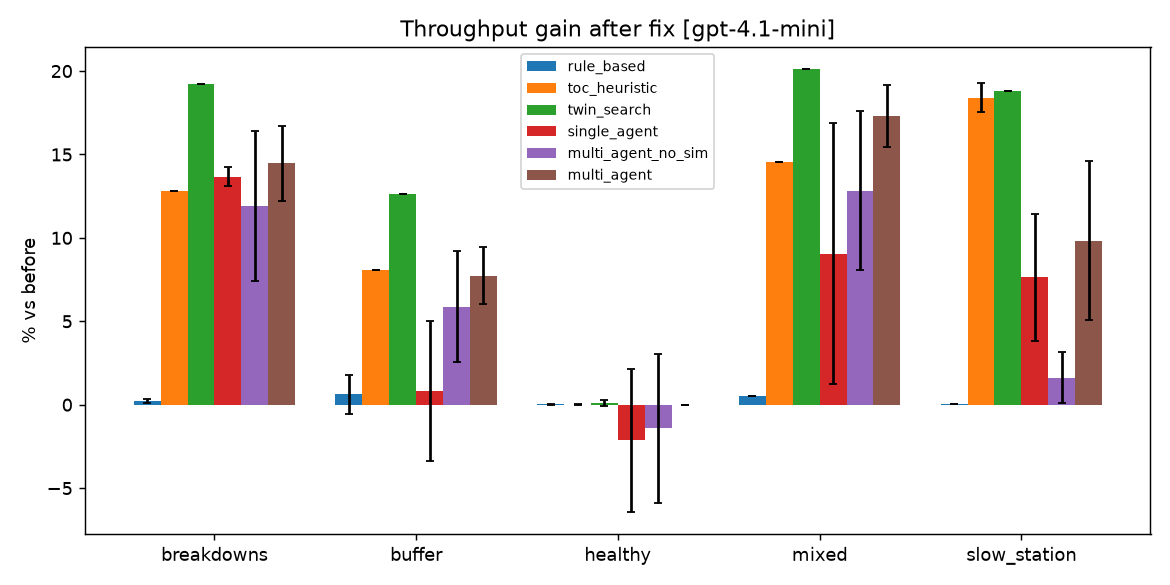
\includegraphics[width=\columnwidth]{gain_pct.png}
\caption{Throughput gain by scenario and system (clean experiment, 95\% CI).}
\label{fig:gain}
\end{figure}

Figure~\ref{fig:gain} shows the same gains with confidence intervals. The intervals of the rule-based, TOC
and twin-search systems are very narrow or collapse to a point in most scenarios, whereas those of the LLM
systems are wider.

\subsection{Against strong non-LLM baselines}
The proposed system does not beat the baselines. Paired over \Npairs{} (scenario, seed) pairs, multi-agent
minus TOC rules is \DiffToc, and minus exhaustive twin search is \DiffTwin. Twin search spends
about \TwinSims{} twin simulations per run and no tokens; multi-agent spends about \TokensMulti{} tokens
per run and tests at most five candidates per round. On this five-station testbed the proposer's shortlist,
not the twin, limits the multi-agent result. Its remaining advantage is a diagnosis and an explanation, which
search does not produce: the judge scores the multi-agent explanation \ExplMulti{} out of 5, against
\ExplTwin{} for twin search and \ExplToc{} for the TOC rules.

\subsection{Does the gate need to trust the evidence?}
Table~\ref{tab:gate} gives the catch rate over bad recommendations. With honest evidence, the trusting gate
catches \CatchHonestTrustMulti\% of multi-agent's bad recommendations. With forged evidence it catches
\CatchForgedTrustMulti\%: it can still reject invalid actions but approves harmful ones that carry good-looking
numbers. The independent gate catches \CatchForgedIndepMulti\% in both cases. It does not reduce
multi-agent's gain (\IndepGainMulti\% vs.\ \GainMulti\%, \IndepAppliedMulti\% of fixes applied), and it improves
the unverified systems (single agent \GainSingle\% to \IndepGainSingle\%, with \IndepAppliedSingle\% of fixes
applied) because the gate itself becomes the verifier.
\begin{table*}[t]
\centering\small
\caption{Gate catch rate (\%) over bad recommendations reaching the gate (count in parentheses). ``Forged'': the bad fix carries the good fix's evidence.}
\label{tab:gate}
\begin{tabular}{lcccc}
\toprule
System & Honest, trusting & Honest, independent & Forged, trusting & Forged, independent \\
\midrule
Naive rule & 60 (20) & 100 (20) & 60 (20) & 100 (20) \\
TOC rules & 60 (20) & 100 (20) & 60 (20) & 100 (20) \\
Twin search & 100 (38) & 100 (38) & 63 (30) & 100 (38) \\
Single agent & 57 (44) & 100 (75) & 57 (44) & 100 (75) \\
Multi-agent, no sim. & 61 (41) & 100 (70) & 61 (41) & 100 (70) \\
Multi-agent + sim. (ours) & 100 (37) & 100 (38) & 63 (30) & 100 (38) \\
\bottomrule
\end{tabular}

\end{table*}

Table~\ref{tab:status} splits the honest-evidence, trusting-gate result by why the recommendation was bad.
Invalid recommendations are caught by every system, because constraint checking is deterministic. Harmful but
valid recommendations are caught only when twin evidence is shown: \HarmCatchMulti\% for the proposed system
(n=\HarmNMulti) and \HarmCatchSingle\% for the single agent (n=\HarmNSingle). This follows from how the
simulated approver is defined, so it verifies the mechanism and is not an independent finding about human
supervisors.
\begin{table}[t]
\centering\small
\caption{Trusting-gate catch rate (\%) by reason the recommendation was bad, stress experiment (count in parentheses).}
\label{tab:status}
\begin{tabular}{lcc}
\toprule
System & Invalid caught (\%) & Harmful caught (\%) \\
\midrule
Naive rule & 100 (12) & 0 (8) \\
TOC rules & 100 (12) & 0 (8) \\
Twin search & 100 (22) & 100 (16) \\
Single agent & 100 (25) & 0 (19) \\
Multi-agent, no sim. & 100 (25) & 0 (16) \\
Multi-agent + sim. (ours) & 100 (21) & 100 (16) \\
\bottomrule
\end{tabular}

\end{table}

\section{Discussion}
\textbf{What the twin buys.} Verification removed every ineffective fix and every false alarm for the
multi-agent system and made its recommendations safe to present, regardless of how good the proposer is.
That property is a consequence of the verification loop and gate, which is why we regard it as the main result.

\textbf{When the LLM may matter.} On this testbed the action grid has only \TwinGrid{} entries, so exhaustive
search costs about \TwinSims{} simulations per run and finds larger gains than the LLM's shortlist. We expect
this to change when the action space grows, for example with more stations, multi-step action sequences or
continuous parameters, because enumeration cost grows with the grid while an LLM proposer's cost does not;
we did not test this, and it is the main reason to repeat the study on larger lines.

\textbf{Why the independent gate matters.} A gate that accepts presented evidence is only as trustworthy as
the process that produced it. An independent gate costs \NReps{} extra paired replications per review and
removes that dependency.

\section{Limitations}
\label{sec:limits}
\begin{itemize}
  \item \textbf{No model mismatch.} The twin that verifies a fix is the simulator that scores it (different
        seeds). The independent gate removes selection bias and forged evidence, not model error. A
        mis-specified-twin experiment exists in the code base but was not run for these results.
  \item \textbf{Synthetic testbed.} One five-station line with four hand-built faults and illustrative
        parameters; no calibration to a real plant.
  \item \textbf{Simulated approver.} The gate is rule-based, never errs and is never persuaded by plausible
        text. No human-gate study was run, and the blind human-review sheet prepared for explanation quality
        was not scored.
  \item \textbf{One model family, \Nseeds{} seeds.} Only \Model{} was evaluated, and confidence intervals are
        wide for small differences; in particular the single-versus-multi-agent accuracy comparison cannot rule
        out a meaningful difference in either direction.
  \item \textbf{Explanation quality} is scored by an LLM judge that sees the reference label and has not been
        validated against human scores~\cite{zheng2023judge}.
\end{itemize}

\section{Conclusion}
Requiring twin verification before recommendation makes LLM supervision measurably safer on this testbed:
fewer ineffective fixes and no false alarms. It does not make it better than a classical rule or exhaustive
search, and its gate must not trust the evidence it is shown. Future work should run the independent gate
under a mis-specified twin, collect real supervisor decisions through the dashboard, evaluate more model
families and seeds, and test larger lines where enumeration is infeasible and a good proposer should matter.

\section*{Reproducibility}
All numbers in this paper are generated from the experiment outputs by a script that writes the table and
macro files included here. Observation seeds are 1--\Nseeds{}, reference seeds 100--104, the Simulation agent
uses seeds 1000+, scoring uses seeds 2000--2019 and the independent gate uses seeds 3000+, so no component
sees another's seeds. LLM responses are cached by model and prompt, which makes reruns reproducible.
\todo{Repository URL and commit hash.}

\bibliographystyle{IEEEtran}
\bibliography{refs}

\end{document}
